\section{Интегрируемость непрерывных и монотонных на отрезке функций по Риману.}

\begin{theorem}[Интегрируемость монотонных функций]
    Если $f(x)$ монотонна на $[a; b]$, то $f(x) \in R[a; b]$
\end{theorem}

\begin{Proof}
   Пусть $f(x)$ неубывает

    1) $f(x) \text{ огр сверху } f(b) \text{ и огр снизу } f(a)$

    2) Предположим противное. Пусть $I^* \neq I_*$:
    \[
        0 < I^* - I_* \leq S_\tau - s_\tau\ \forall \tau = \Sum{i = 1}{n}(M_i - m_i)|\D x_i|\leq d(\tau)\Sum{i = 1}{n}(M_i - m_i) =
    \]
    \[
        = d(\tau)\Sum{i = 1}{n}(f(x_i) - f(x_{i-1})) = d(\tau)(f(b) - f(a)) \text{ --- сколь угодно малое число}
    \]
    $\D x_i = [x_{i-1}; x_i]$

    Возьмем $\tau$: $d(\tau) < \frac{I^* - I_*}{f(b) - f(a)}\cdot\frac{1}{2}$

    \[
        d(\tau)(f(b) - f(a)) < (I^* - I_*)\cdot\frac{1}{2}
    \]

    \[
        0 < I^* - I_* \leq (I^* - I_*)\cdot\frac{1}{2},\ \bot
    \]
\end{Proof}

\begin{definition}[Определение 1]
    $f(x)$ называется равномерно непрерывной на $E$, если:
    \[
        \forall \eps > 0~ \exists\delta > 0 ~\forall x_1, x_2 \in E: |x_1 - x_2| < \delta \Rightarrow |f(x_1) - f(x_2)| < \eps
    \]
\end{definition}

\begin{definition}[Определение 2]
    $f(x)$ непрерывна на E, если\\
    \[
        \forall x_1 \in E~ \forall \eps > 0~ \exists\delta > 0 ~\forall x_2 \in E: |x_1 - x_2| < \delta \Rightarrow |f(x_1) - f(x_2)| < \eps
    \]

\end{definition}

\begin{consequence}
    Определение 1 $\implies$ Определение 2

    Определение 2 $\nRightarrow$ Определение 1 $\left(f(x) = \frac{1}{x} \text{ на } (0, 1),\ x_n = \frac{1}{n},\ |x_{n+1} - x_n| \xrightarrow[n \to \infty ]{} 0 \right)$
\end{consequence}

\begin{theorem}[Кантора]
    Если $f(x)$ непр на [a; b], то $f(x)$ равномерное непр на отрезке
\end{theorem}

\begin{Proof}
    От противного\\
    $\exists \eps_0~ \forall \delta > 0~ \exists x_1(\delta), x_2(\delta)\in [a; b]: |x_1 - x_2| < \delta$ и $|f(x_1) - f(x_2)| > \eps_0$\\
    Возьмем $\delta = \frac{1}{n}~$\\$ \exists x_{1, n}, x_{2, n}: |x_{1, n} - x_{2, n}| < \frac{1}{n}$ и $|f(x_{1, n}) - f(x_{2, n})| > \eps_0$\\
    $\{x_{1, n}\}, \{x_{2, n}\} \subset [a; b]$\\
    По теореме Б-В:\\
    $\exists k_n~~: x_{1, k_n} \implunder{n \rightarrow \infty} x_1$\\
    По теореме Б-В: $x_{2, k_n}$\\
    $\exists k_{l_n}:~~ x_{2, k_{l_n}} \implunder{n \rightarrow \infty} x_2 \in [a; b]$\\
    $x_{1, k_{l_n}}\implunder{n \rightarrow \infty} x_1 \in [a; b]$

    \begin{center}
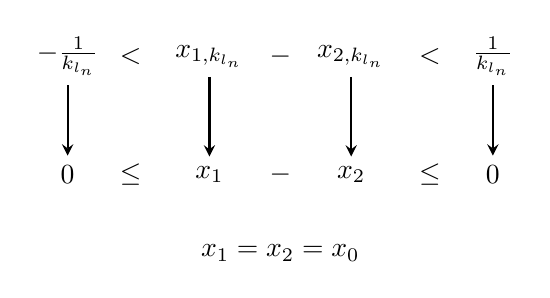
\begin{tikzpicture}[>=stealth, node distance=1.5cm]
    % Верхняя строка
    \node (A1) at (0,0) {$-\frac{1}{k_{l_n}}$};
    \node (lt1) at (0.8,0) {$<$};
    \node (A2) at (1.8,0) {$x_{1,k_{l_n}}$};
    \node (minus) at (2.7,0) {$-$};
    \node (A3) at (3.6,0) {$x_{2,k_{l_n}}$};
    \node (lt2) at (4.6,0) {$<$};
    \node (A4) at (5.4,0) {$\frac{1}{k_{l_n}}$};

    % Нижняя строка (предельные значения)
    \node (B1) at (0,-1.5) {$0$};
    \node (le1) at (0.8,-1.5) {$\leq$};
    \node (B2) at (1.8,-1.5) {$x_1$};
    \node (minus2) at (2.7,-1.5) {$-$};
    \node (B3) at (3.6,-1.5) {$x_2$};
    \node (le2) at (4.6,-1.5) {$\leq$};
    \node (B4) at (5.4,-1.5) {$0$};

    % Стрелки перехода к пределу
    \draw[->, thick] (A1) -- (B1);
    \draw[->, thick] (A2) -- (B2);
    \draw[->, thick] (A3) -- (B3);
    \draw[->, thick] (A4) -- (B4);

    % Итоговое равенство
    \node at (2.7, -2.5) {$x_1 = x_2 = x_0$};
\end{tikzpicture}
\end{center}
    Непрерывность по Гейне в точке $x_0 \in [a, b]$\\
    $f(x_{1, k_{l_n}})\implunder{n \rightarrow \infty} f(x_0) \in [a; b]$\\
    $f(x_{2, k_{l_n}})\implunder{n \rightarrow \infty} f(x_0) \in [a; b]$\\
    Противоречие с отрицанием, у нас для любых двух значений функции должен был найтись некий $\eps_0 > 0$, но разность между элементами сходится к 0.
\end{Proof}

\begin{theorem}[Теор2]
    Если $f(x)$ непр на [a; b], то $f(x) \in R[a; b]$\\   
\end{theorem}

\begin{Proof}
    По критерию Дарбу

    1) Огр выполнена

    2) Докажем от противного

    $0 < I^* - I_* \leq_\forall\tau S_\tau - s_\tau = Sum{i = 1}{n}(M_i - m_i)|\D x_i|$\\
    $\exists \xi_i, \eta_i \in \D x_i: |\xi_i - \eta_i| \leq d(\tau)< \delta$\\
    $Sum{i = 1}{n}(M_i - m_i)|\D x_i| = Sum{i = 1}{n}(f(\xi_i) - f(\eta_i))|\D x_i| < \eps \Sum{i = 1}{n}|\D x_i|$\\
    Возьмем $\eps = \frac{I^* - I_*}{b - a} \cdot \frac{1}{2} \rightarrow \delta(\eps)$\\
    Построим по полученной $\delta(\eps) d(\tau)$
    $\eps \Sum{i = 1}{n}|\D x_i| = \eps(b - a) = \frac{I^* - I_*}{2}$ - Противоречие\\
    $0 < I^* - I_* < \frac{I^* - I_*}{2}$
\end{Proof}



